\documentclass[12pt,a4paper]{report}
\usepackage{nomencl}


\usepackage{arabtex}
\usepackage{utf8}
\setcode{utf8}

\usepackage[utf8]{inputenc}
%\usepackage[]{babel}
\usepackage[T1]{fontenc}
%\usepackage{amsmath}
\usepackage{pdfpages}
\usepackage{enumitem}
\usepackage{amsfonts}
\usepackage{xcolor}
%\usepackage{amssymb}
%\usepackage{natbib}
\usepackage{xspace}
\usepackage{graphicx}
 \usepackage{comment} 
% \usepackage[acronym]{glossaries}
%\usepackage{float}
\usepackage{tabularx}
\usepackage{array}
%\usepackage{arabtex}
\usepackage{rotating}
\usepackage{tikz}
%\usepackage{cite}
\usepackage{amsmath,amssymb,amsfonts}
\usepackage{lmodern}
\usepackage{xspace}
\usepackage{multicol}
\usepackage{lipsum}
\usepackage{pgfplots}
\usetikzlibrary{plotmarks}
\usepackage{float}
\usepackage{geometry}
%\usepackage{utf8}
%\setcode{utf8}
\usepackage{multirow}
\usepackage{setspace}
\usepackage[Glenn]{ fncychap }
\usepackage{fancyhdr}
\usepackage{subcaption}
\usepackage{algorithm}
\usepackage[sort]{acronym}
\usepackage{algpseudocode}
\definecolor{accessblue}{RGB}{0,105,154}
\definecolor{accessdarkblue}{RGB}{0,67,109}
\definecolor{accesshighlight}{RGB}{38,205,197}
\definecolor{col16}{HTML}{C0392B }
\definecolor{col30}{HTML}{1E8449}
\definecolor{col17}{HTML}{F7DC6F}
\definecolor{col18}{HTML}{F778A1}
\definecolor{col21}{HTML}{9B59B6}
\definecolor{col22}{HTML}{7F8C8D}
\definecolor{col9}{HTML}{4b1129}
\definecolor{col0}{HTML}{3278ca} % blue 1
\definecolor{col10}{HTML}{9e1958}
\definecolor{col1}{HTML}{259b9c} % green 2
\definecolor{col11}{HTML}{bc5484}
\definecolor{col2}{HTML}{ff8839} % orange 3
\definecolor{col12}{HTML}{f0780d}
\definecolor{col6}{RGB}{0,105,154}
\definecolor{col13}{HTML}{d35d03}
\definecolor{col4}{HTML}{5358d3} % blue 5
\definecolor{col14}{HTML}{b1b52a}
\definecolor{col5}{HTML}{ffbd50} % orange 6
\definecolor{col3}{HTML}{57d7cf}
\definecolor{col7}{HTML}{5e9289}
\definecolor{col8}{HTML}{64b1aa}

\pagestyle{fancy}
\lhead{\leftmark}
\rhead{}
\geometry{left=2.5cm, right=2cm, top=2.5cm, bottom=2.5cm}
\onehalfspacing
\let\mylistof\listof
\renewcommand\listof[2]{\mylistof{algorithm}{List of algorithms}}
%\renewcommand\listof[5]{\mylistof{acronym}{Acronyms}}
%\makeglossaries
%\usepackage{acronym}

\begin{document}
\thispagestyle{empty}
\setlength{\fboxrule}{0.4mm}
\setlength{\fboxsep}{3mm}
N$^0$ d'ordre....../FT/UMBB/2024
\begin{center}
 People's Democratic Republic of Algeria\\
Ministry of Higher Education and Scientific Research\\
\textbf{University M'Hamed Bougara of Boumerdes}\\
\end{center}
\begin{figure}[H]
  \centering
  
\includegraphics[width=0.3\linewidth]{UMBB.png}
\end{figure}
\begin{center}
\textbf{Faculty of Technology} \\
%\textbf{Systems Engineering and Telecommunications Laboratory} \\
\end{center}
\begin{center}
\begin{LARGE}
\textbf{PHD DISSERTATION}\\
\end{LARGE}\vfill
\begin{large} PRESENTED BY: Your Name  \\
%\textbf{Ph.D Student}\\
In Partial Fulfilment Of The Requirements For The Degree Of \\
\textbf{Doctorat }\\
\end{large}
\end{center}
\vfill
\textbf{Field: Biomedical Engenering} \\
\textbf{Option: Biomedical Intrumentation} \\
\begin{center}
\textbf{TITLE}
\end{center}\\\\
\fbox{\begin{minipage}[c]{0.9\linewidth}
\begin{center}
\begin{large}
\textbf{X-ray image analysis for Knee Osteoarthritis detection}
\end{large}
\end{center}
\end{minipage}}
%\rule{1\textwidth}{2pt}\vfill
\vfill







JURY MEMBERS:\\

\begin{center}
\begin{tabular}{lllll}
Pr. Name  & Professor & University of  & President\\
Dr. Name  & Professor & University of  & Examiner\\
Dr. Name  & Professor & University of  & Examiner\\
\end{tabular}
\end{center}
\begin{center}
Academic Year: 2025/2026
\end{center}
%2023/2024
\newpage

\chapter*{Acknowledgements}
\thispagestyle{empty}

%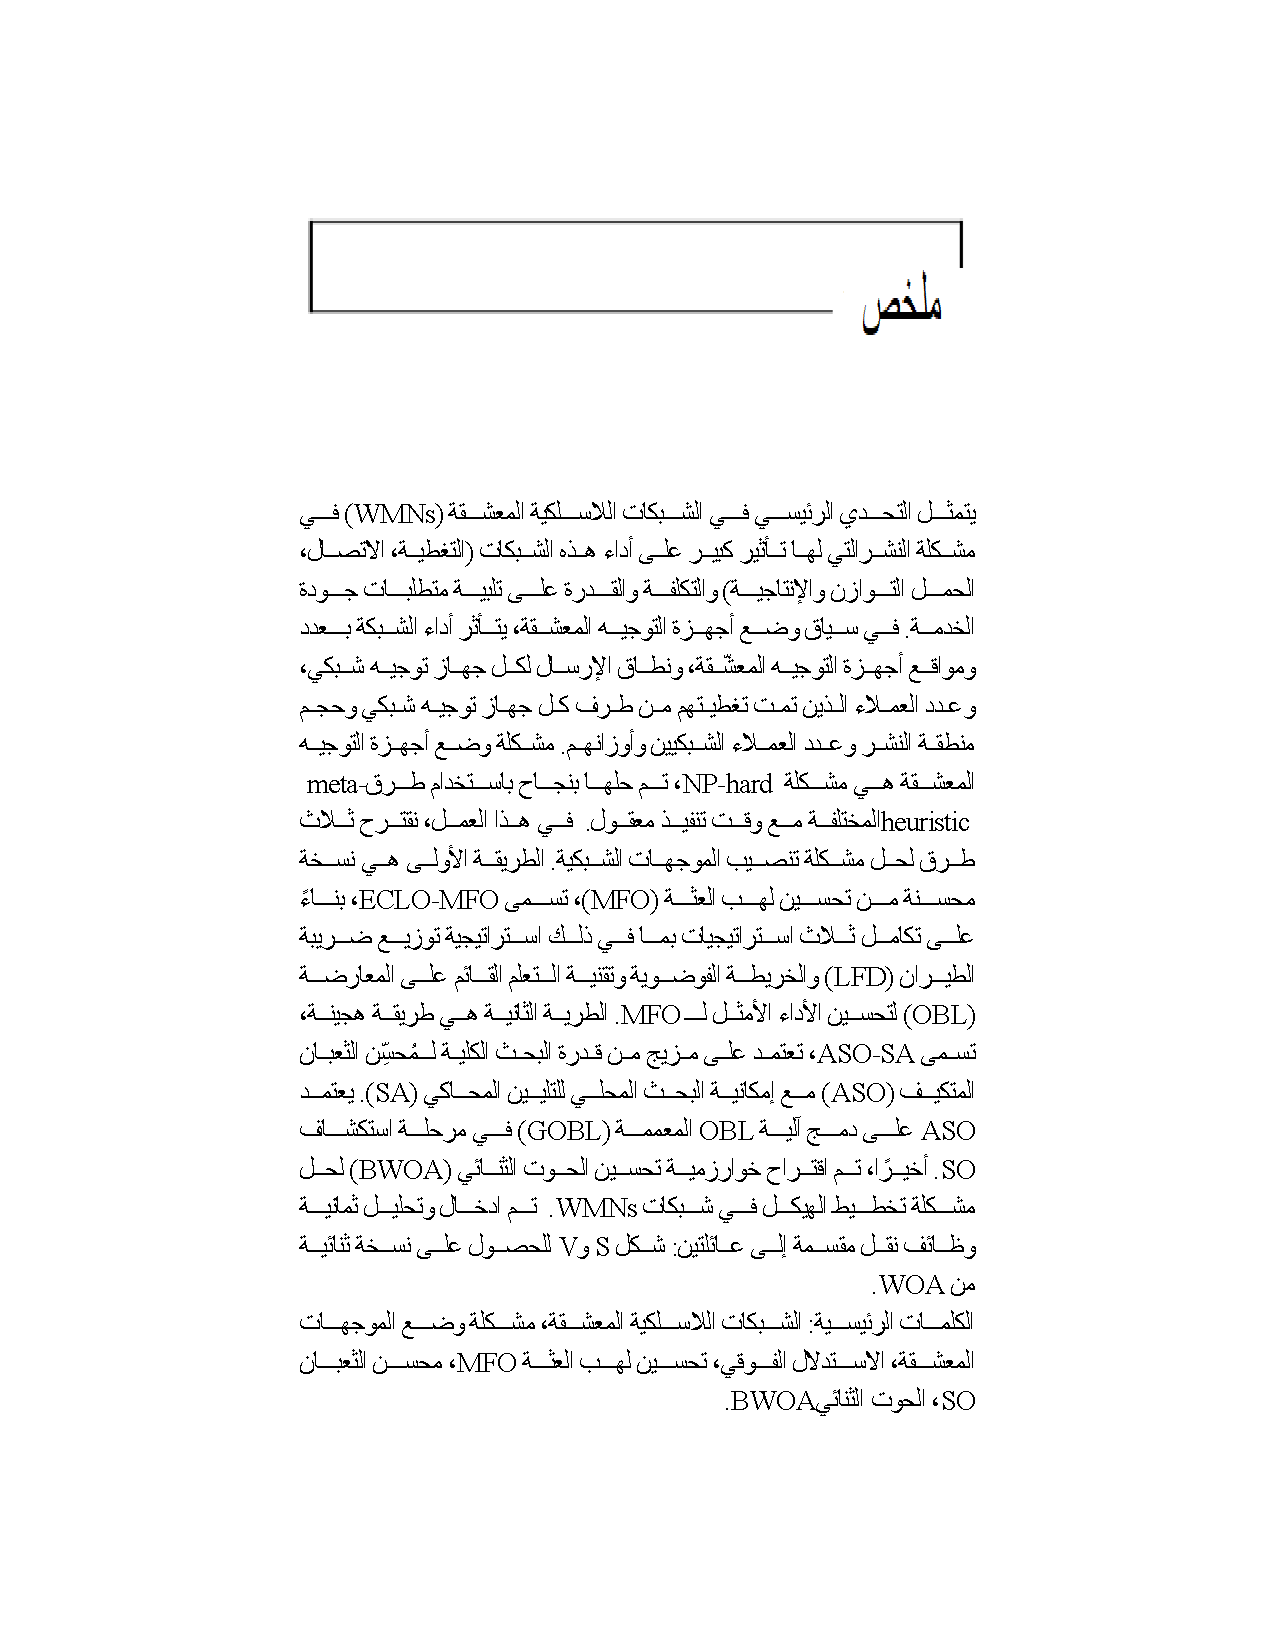
\includepdf[pages={1}]{abss - Copy - Copy (2).pdf}
%\setcounter{page}{0}

\chapter*{\<الملخص>}
\thispagestyle{empty}
\begin{arabtex}
الملخص الملخص الملخص الملخص الملخص الملخص الملخص الملخص الملخص الملخص الملخص الملخص الملخص الملخص الملخص الملخص الملخص الملخص الملخص 

\vspace{5mm} %5mm vertical space
\textbf{الكلمات اللمفتاحية}:

\end{arabtex}


\chapter*{Abstract}
\thispagestyle{empty}
\begin{sloppypar}
text text text text text text text text text text text text text text text text text text text text text text text text text text text 


\textbf{Keywords}: text text text
\end{sloppypar}



\chapter*{Résumé}
\thispagestyle{empty}
% 
text text text text text text text text text text text text text text text text text text text text text text text text text text text text text text text



\textbf{Mots clés}: text text text
\newpage
\pagenumbering{Roman}
\tableofcontents
\listoffigures
\listoftables
\listofalgorithms



\makenomenclature  % Enable nomenclature

% Redefine the nomenclature title
\renewcommand{\nomname}{Acronyms }


%\addcontentsline{toc}{section}{Acronyms} % Add it to the table of contents
\printnomenclature % Print the list of abbreviations


\nomenclature{\textbf{DWT}}{Discret Wavelet Transform}
\nomenclature{\textbf{}}{}
\nomenclature{\textbf{}}{}
\nomenclature{\textbf{}}{}
\nomenclature{\textbf{}}{}
\nomenclature{\textbf{}}{}







\chapter*{General Introduction}
\addcontentsline{toc}{chapter}{General Introduction}
\markboth{\MakeUppercase{General Introduction}}{\MakeUppercase{General Introduction}}
\pagenumbering{arabic}
\begin{sloppypar}


\newpage
\chapter{}
%\pagenumbering{arabic}
\section{Introduction}
text text text text text text text text text text text text text text text text text text text text text text text text text text text text text text text text text text text text text text text text text text text text text text text text text text text text text text text text text text text text text text text text text text text text text text text text 
\cite{patil2013medical}   \cite{pham2000current}.

\section{}
\section{}


\section{Conclusion}

%%%%%%%%%%%%%%%%%%%%%%%%%%%%%%%%%%%%%%%%%%%%%%%
%%%%%%%%%%%%%%%%%%%%%%%%%%%%%%%%%%%%%%%%%%%%%%%
%%%%%%%%%%%%%%%%%%%%%%%%%%%%%%%%%%%%%%%%%%%%%%%
\chapter{Related work}
\setcounter{secnumdepth}{3}
\section{Introduction}
 
\subsection{aaaaa}
text text text text text text text text text text text text text text text text text text text text text text text text text text text text text text text text text text text text text text text text text text text text text text text text text text text text text text text text text text text text text text text text text text text text text text text text 
\begin{figure}[H]
    \centering
    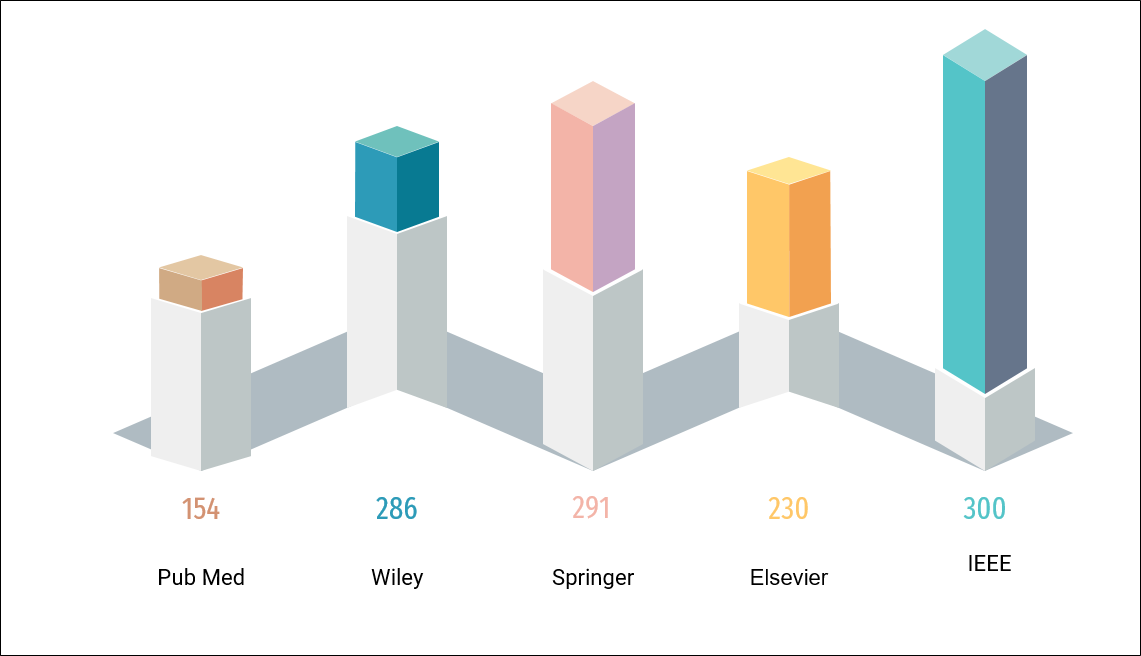
\includegraphics[width=\textwidth]{img1.png} % Remplacez par le nom de votre fichier image
    \caption{SDistribution of research papers by publisher}
    \label{fig:mon_image}
\end{figure}



\section{Conclusion}

%\documentclass{article}
\usepackage{tikz}
\usetikzlibrary{arrows,shapes,positioning,shadows,trees}

\begin{document}

\tikzset{
  basic/.style  = {draw, text width=2cm, drop shadow, font=\sffamily, rectangle},
  root/.style   = {basic, thin, align=center,
               fill=gray!45},
  level 2/.style = {basic, thin,align=center, fill=gray!30,
               text width=8em},
  level 3/.style = {basic, thin, align=left, fill=gray!20, text width=6.5em, node distance = 40pt}
}
\begin{tikzpicture}[
  level 1/.style={sibling distance=40mm},
  edge from parent/.style={->,draw},
  >=latex]

% root of the the initial tree, level 1
\node[root] {Population-based meta-heuristics}
% The first level, as children of the initial tree
  child {node[level 2] (c1) {Swarm intelligence}}
  child {node[level 2] (c2) {Physical-based}}
  child {node[level 2] (c3) {Distributed Key Agreement}};

% The second level, relatively positioned nodes
\begin{scope}[every node/.style={level 3}]
\node [below of = c1, xshift=15pt] (c11) {Pairwise Keys};
\node [below of = c11] (c12) {Broadcast Secrets};
\node [below of = c12] (c13) {Keys Hierarchy};

\node [below of = c2, xshift=15pt] (c21) {Membership driven Re-Keying};
\node [below of = c21] (c22) {Time driven Re-Keying};

\node [below of = c3, xshift=15pt] (c31) {Ring-based Cooperation};
\node [below of = c31] (c32) {Hierarchical Cooperation};
\node [below of = c32] (c33) {Broadcast Cooperation};
\end{scope}

% lines from each level 1 node to every one of its "children"
\foreach \value in {1,2,3}
  \draw[->] (c1.195) |- (c1\value.west);

\foreach \value in {1,2}
  \draw[->] (c2.195) |- (c2\value.west);

\foreach \value in {1,2,3}
  \draw[->] (c3.195) |- (c3\value.west);
\end{tikzpicture}

\end{document}
\chapter{Detection of knee osteoarthritis based on texture analysis methods.}

\section{Introduction}

\section{aaaaaa}
\subsection{aaaaa}
 
\begin{itemize}
    \item item 1
\item item 2
\item item 3
\item item 4
\end{itemize}
\subsection{aaaaa}
\subsubsection{aaaaa}

\subsubsection{aaaaa}


\section{Conclusion}



\chapter*{General conclusion}
%\pagenumbering{arabic}

\bibliographystyle{unsrt}
\bibliography{mabiblio}

\end{document}